\documentclass[notitlepage]{article}
\usepackage{ctex}
\usepackage{amsmath}
\usepackage{amssymb}
\usepackage{indentfirst}
\usepackage{graphicx}
\usepackage{float}
\usepackage{subfig}
\usepackage{overpic}
\usepackage[a4paper, scale=0.85]{geometry}

\title{实验三\ 神经网络}
\author{}
\date{}

\setlength{\parindent}{2em}
\linespread{2}

\begin{document}

\maketitle

\vspace{-7em}

\section{问题描述}

利用神经网络算法对MNIST数据集进行分类

\section{实现步骤与流程}

BP算法通过链式法则将误差对参数的梯度逐级传播,并通过梯度下降算法对参数进行优化

\subsection*{加载数据集}

实验提供的MNIST数据集文件为.idx3-ubyte和.idx1-ubyte格式,需要对读取到的
二进制序列进行处理,转化为numpy可以进行运算的ndarray的格式

\subsection*{定义基础模块}

神经网络可能由多个模块构成,为了简化网络模型的构建过程,需要对神经网络中的模块概念
进行封装,并定义模块的前向传播以及反向传播机制,本次实验实现了多种基本模块,包括
全连接层(Linear)、标准化层(LayerNormalization)以及常见的激活函数relu层、
sigmoid层、tanh层以及softma层,并提供了简单的序列神经网络模块(Sequence)用于
堆叠各种模块形成网络

\subsection*{定义损失函数}

为了对网络中的参数进行优化,还需要定义损失函数,包括损失函数的计算以及梯度的回传。
本次实验提供了交叉熵损失函数(CrossEntropy)用于多分类任务的优化

\subsection*{构建训练网络}

在初始化数据集以及构建好神经网络后,即可对网络中的参数进行学习训练。本次实验采用小批次梯度
下降算法,为了加快网络的收敛速度的同时保证网络收敛的稳定性,实验中采用了学习率的指数衰减策略,
并且为了减少网络过拟合的可能,实验中实现了网络的提前体制(early-stop)。在训练过程中记录
网络模型在训练集以及验证集上的平均损失函数以及准确率的历史数据,训练结束后可视化历史数据,观察
网络的训练过程

\section{实验结果与分析}

由于实验要求的MindSpore框架相关的资料较为匮乏,因此本次实验采取深度学习框架pytorch
与实验中的算法进行对比。pytorch是一个开源的python深度学习库,可以用于构建能够自动
求导的神经网络。

以下是实验中构建的神经网络的训练历史和相同结构的网络在pytorch下的训练历史

\begin{figure*}[htbp]
	\centering
	\subfloat[历史数据(实验)]{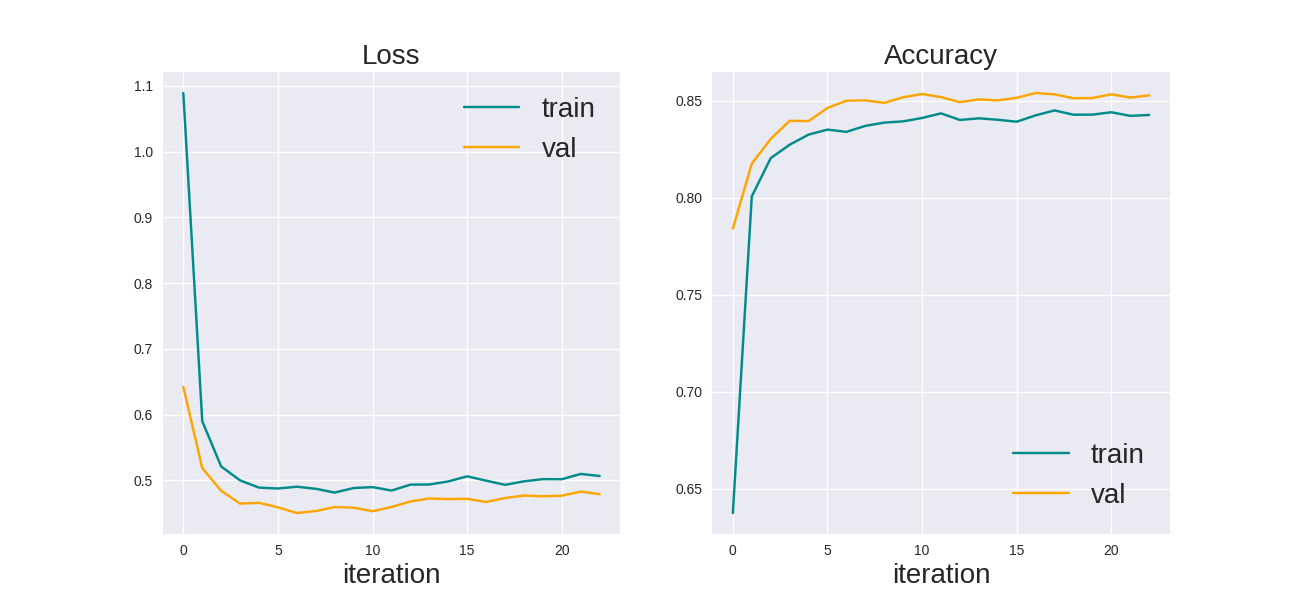
\includegraphics[width=.85\columnwidth]
    {../imgs/mine/history.png}}\\
	\subfloat[历史数据(pytorch)]{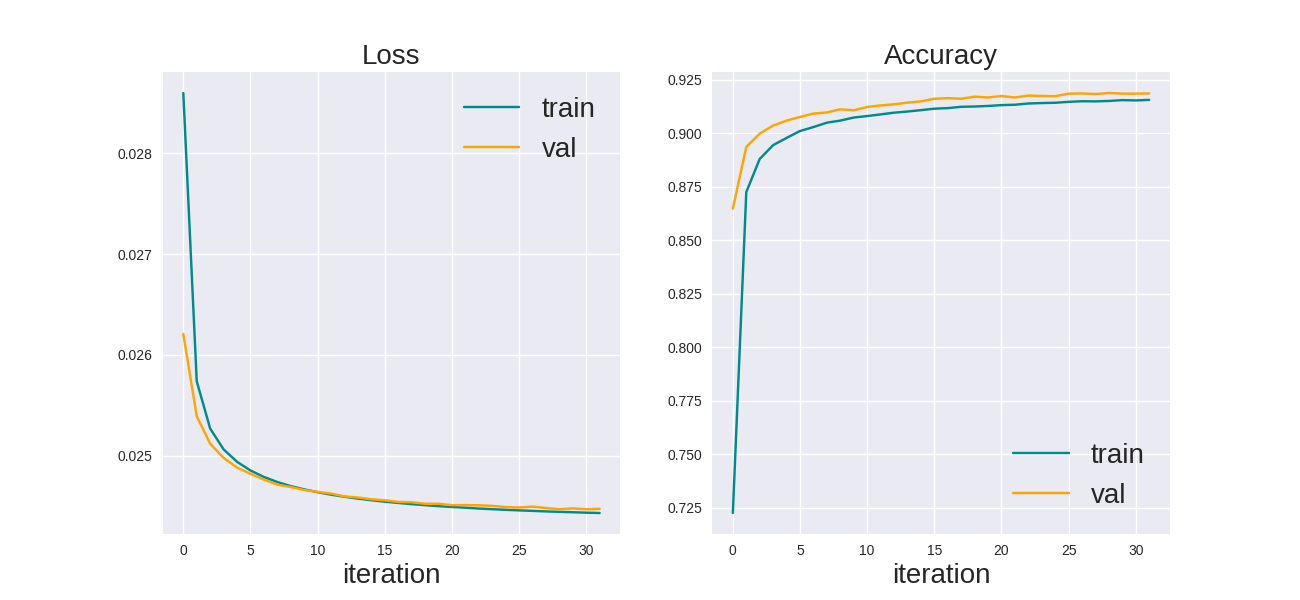
\includegraphics[width=.85\columnwidth]
    {../imgs/pytorch/history.png}}
	\caption{神经网络训练历史}
\end{figure*}

可以看出,随着训练轮数的增加,网络模型在分类的准确率上不断上升最终达到收敛。与pytorch的算法相比,
实验的算法最终的收敛准确率较低,在85\%左右,而pytorch最终的准确率可以达到接近92\%,
并且在实验算法每个轮次需要约1.6s的运行时间,而pytorch每个轮次需要1.2s的运行时间,在时间效率上更高。

经过实际测试,本次实验采用的单层网络结构在训练效率以及准确率上的综合表现较好。

\section{MindSpore学习使用心得体会}

由于本次实验并未采用MindSpore,此部分用pytorch的学习使用心得体会来代替。

本次实验中调用了pytorch中的以下算法接口
\begin{itemize}
    \item 神经网络模块(nn)
    \item 数据集接口(utils data Dataset、DataLoader)
    \item SGD优化器(optim SGD)
    \item 学习率指数衰减(optim lr\_scheduler ExponentialLR)
\end{itemize}

作为实验算法的对照算法,pytorch提供的算法接口方便调用,并且执行效率较高,能够高效地实现实验的需求。

\newpage

\section{代码附录}

\begin{figure*}[h]
    \centering
    \includegraphics*[width=\columnwidth]{../imgs/code.png}
    \caption{部分代码截图}
\end{figure*}

\end{document}